\subsection{Convolutional Neural Networks: Application}

Welcome to Course 4's second assignment! You will:
\begin{itemize}
\item Implement helper functions that you will use when implementing a TensorFlow model
\item Implement a fully functioning ConvNet using TensorFlow
\end{itemize}

After this assignment you will be able to:
\begin{itemize}
\item Build and train a ConvNet in TensorFlow for a classification problem
\end{itemize}

We assume here that you are already familiar with TensorFlow. If you are not, please refer the TensorFlow Tutorial of the third week of Course 2 (``Improving deep neural networks").


\subsubsection{TensorFlow model}
In the previous assignment, you built helper functions using numpy to understand the mechanics behind convolutional neural networks. Most practical applications of deep learning today are built using programming frameworks, which have many built-in functions you can simply call.

As usual, we will start by loading in the packages.

\begin{minted}{python}
import math
import numpy as np
import h5py
import matplotlib.pyplot as plt
import scipy
from PIL import Image
from scipy import ndimage
import tensorflow as tf
from tensorflow.python.framework import ops
from cnn_utils import *

np.random.seed(1)
\end{minted}

Run the next cell to load the ``SIGNS" dataset you are going to use.
\begin{minted}{python}
# Loading the data (signs)
X_train_orig, Y_train_orig, X_test_orig, Y_test_orig, classes = load_dataset()
\end{minted}

As a reminder, the SIGNS dataset is a collection of 6 signs representing numbers from 0 to 5.
\clearpage
\begin{figure}[h]
\begin{center}
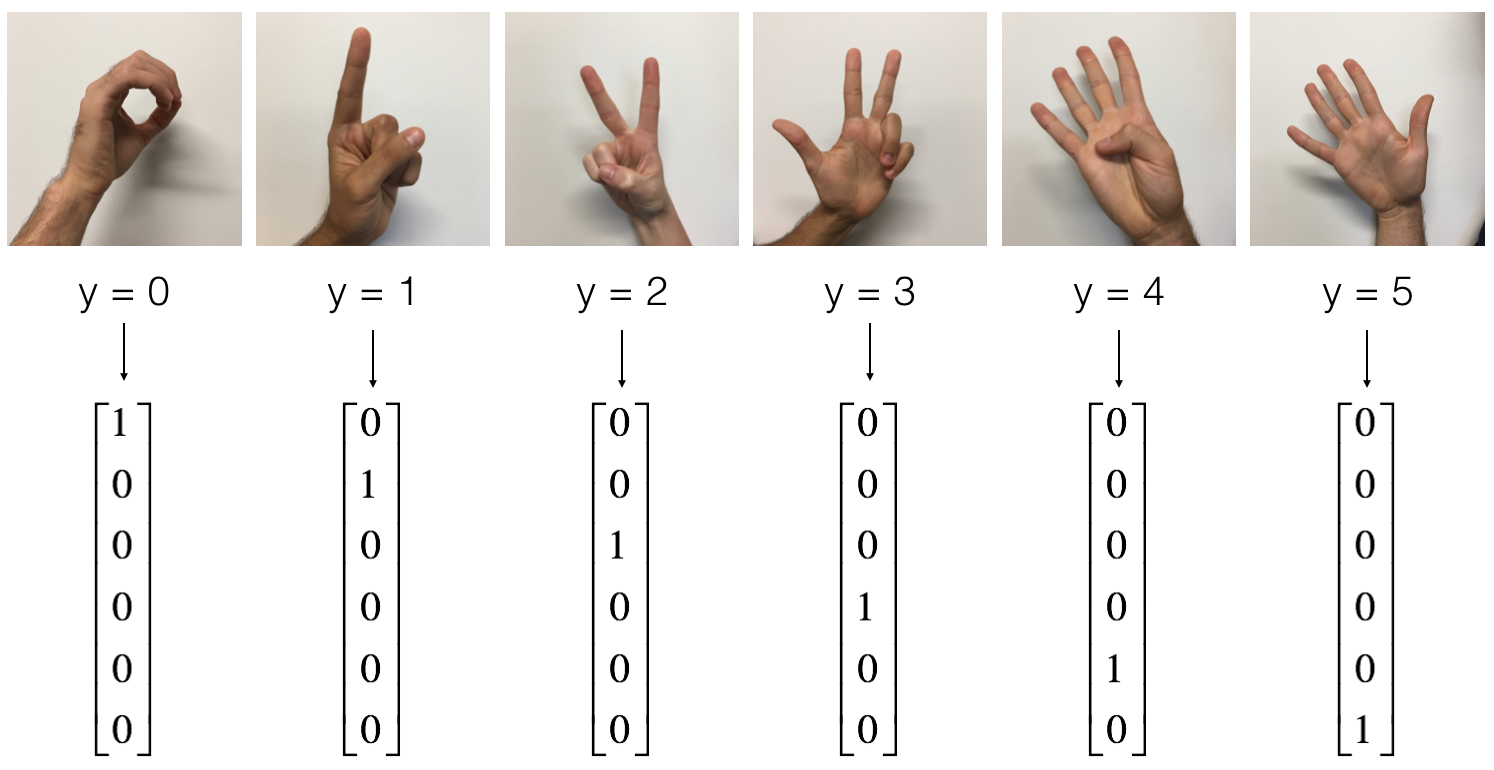
\includegraphics[width=0.8\textwidth]{course4/SIGNS_dataset}
\end{center}
\end{figure}

\begin{minted}{python}
# Example of a picture
index = 6
plt.imshow(X_train_orig[index])
print ("y = " + str(np.squeeze(Y_train_orig[:, index])))
\end{minted}
y = 2
\begin{figure}[h]
\begin{center}
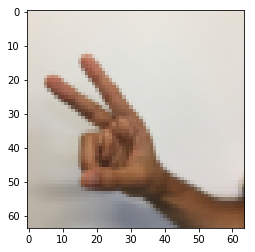
\includegraphics[width=0.3\textwidth]{course4/dataset_example}
\end{center}
\end{figure}


In Course 2, you had built a fully-connected network for this dataset. But since this is an image dataset, it is more natural to apply a ConvNet to it.

To get started, let's examine the shapes of your data.
\begin{minted}{python}
X_train = X_train_orig/255.
X_test = X_test_orig/255.
Y_train = convert_to_one_hot(Y_train_orig, 6).T
Y_test = convert_to_one_hot(Y_test_orig, 6).T
print ("number of training examples = " + str(X_train.shape[0]))
print ("number of test examples = " + str(X_test.shape[0]))
print ("X_train shape: " + str(X_train.shape))
print ("Y_train shape: " + str(Y_train.shape))
print ("X_test shape: " + str(X_test.shape))
print ("Y_test shape: " + str(Y_test.shape))
conv_layers = {}
\end{minted}

\begin{minted}{python}
#output
number of training examples = 1080
number of test examples = 120
X_train shape: (1080, 64, 64, 3)
Y_train shape: (1080, 6)
X_test shape: (120, 64, 64, 3)
Y_test shape: (120, 6)
\end{minted}


\subsubsection{Create placeholders}

TensorFlow requires that you create placeholders for the input data that will be fed into the model when running the session.

{\textbf{Exercise}}: Implement the function below to create placeholders for the input image X and the output Y. You should not define the number of training examples for the moment. To do so, you could use ``None" as the batch size, it will give you the flexibility to choose it later. Hence X should be of dimension {\textbf{[None, n\_H0, n\_W0, n\_C0]}} and Y should be of dimension {\textbf{[None, n\_y]}}.  \href{https://www.tensorflow.org/api_docs/python/tf/placeholder}{Hint}.
\begin{minted}{python}
# GRADED FUNCTION: create_placeholders
def create_placeholders(n_H0, n_W0, n_C0, n_y):
    """
    Creates the placeholders for the tensorflow session.
    
    Arguments:
    n_H0 -- scalar, height of an input image
    n_W0 -- scalar, width of an input image
    n_C0 -- scalar, number of channels of the input
    n_y -- scalar, number of classes
        
    Returns:
    X -- placeholder for the data input, of shape [None, n_H0, n_W0, n_C0] and dtype "float"
    Y -- placeholder for the input labels, of shape [None, n_y] and dtype "float"
    """

    ### START CODE HERE ### (≈2 lines)
    X = tf.placeholder(tf.float32, shape=(None, n_H0, n_W0, n_C0))
    Y = tf.placeholder(tf.float32, shape=(None, n_y))
    ### END CODE HERE ###
    
    return X, Y
\end{minted}

\begin{minted}{python}
X, Y = create_placeholders(64, 64, 3, 6)
print ("X = " + str(X))
print ("Y = " + str(Y))

#output
X = Tensor("Placeholder:0", shape=(?, 64, 64, 3), dtype=float32)
Y = Tensor("Placeholder_1:0", shape=(?, 6), dtype=float32)
\end{minted}



\subsubsection{Initialize parameters}

You will initialize weights/filters $W1$ and $W2$ using ``tf.contrib.layers.xavier\_initializer(seed = 0)''. You don't need to worry about bias variables as you will soon see that TensorFlow functions take care of the bias. Note also that you will only initialize the weights/filters for the conv2d functions. TensorFlow initializes the layers for the fully connected part automatically. We will talk more about that later in this assignment.

{\textbf{Exercise}}: Implement initialize\_parameters(). The dimensions for each group of filters are provided below. Reminder - to initialize a parameter $W$ of shape [1,2,3,4] in Tensorflow, use:
\begin{minted}{python}
W = tf.get_variable("W", [1,2,3,4], initializer = ...)
\end{minted}
\href{https://www.tensorflow.org/api_docs/python/tf/get_variable}{More Info}.

\begin{minted}{python}
# GRADED FUNCTION: initialize_parameters
def initialize_parameters():
    """
    Initializes weight parameters to build a neural network with tensorflow. The shapes are:
                        W1 : [4, 4, 3, 8]
                        W2 : [2, 2, 8, 16]
    Returns:
    parameters -- a dictionary of tensors containing W1, W2
    """
    
    tf.set_random_seed(1)                              # so that your "random" numbers match ours
        
    ### START CODE HERE ### (approx. 2 lines of code)
    W1 = tf.get_variable("W1", [4, 4, 3, 8], initializer =tf.contrib.layers.xavier_initializer(seed = 0))
    W2 = tf.get_variable("W2", [2, 2, 8, 16], initializer =tf.contrib.layers.xavier_initializer(seed = 0))
    ### END CODE HERE ###

    parameters = {"W1": W1,
                  "W2": W2}
    
    return parameters
\end{minted}



\subsubsection{Forward propagation}
In TensorFlow, there are built-in functions that carry out the convolution steps for you.
\begin{itemize}
\item {\textbf{tf.nn.conv2d(X,W1, strides = [1,s,s,1], padding = 'SAME')}}: given an input $X$ and a group of filters $W1$, this function convolves $W1$'s filters on X. The third input ([1,s,s,1]) represents the strides for each dimension of the input (m, n\_H\_prev, n\_W\_prev, n\_C\_prev). You can read the full documentation \href{https://www.tensorflow.org/api_docs/python/tf/nn/conv2d}{here}

\item {\textbf{tf.nn.max\_pool(A, ksize = [1,f,f,1], strides = [1,s,s,1], padding = 'SAME')}}: given an input A, this function uses a window of size (f, f) and strides of size (s, s) to carry out max pooling over each window. You can read the full documentation \href{https://www.tensorflow.org/api_docs/python/tf/nn/max_pool}{here}

\item {\textbf{tf.nn.relu(Z1)}}: computes the elementwise ReLU of Z1 (which can be any shape). You can read the full documentation \href{https://www.tensorflow.org/api_docs/python/tf/nn/relu}{here.}

\item {\textbf{tf.contrib.layers.flatten(P)}}: given an input P, this function flattens each example into a 1D vector it while maintaining the batch-size. It returns a flattened tensor with shape [batch\_size, k]. You can read the full documentation \href{https://www.tensorflow.org/api_docs/python/tf/contrib/layers/flatten}{here.}

\item {\textbf{tf.contrib.layers.fully\_connected(F, num\_outputs)}}: given a the flattened input F, it returns the output computed using a fully connected layer. You can read the full documentation \href{https://www.tensorflow.org/api_docs/python/tf/contrib/layers/fully_connected}{here.}
\end{itemize} 

In the last function above (``tf.contrib.layers.fully\_connected''), the fully connected layer automatically initializes weights in the graph and keeps on training them as you train the model. Hence, you did not need to initialize those weights when initializing the parameters. 


{\textbf{Exercise}}:

Implement the ``forward\_propagation'' function below to build the following model: \emph{CONV2D -> RELU -> MAXPOOL -> CONV2D -> RELU -> MAXPOOL -> FLATTEN -> FULLYCONNECTED}. You should use the functions above. 

In detail, we will use the following parameters for all the steps:
\begin{itemize}
\item Conv2D: stride 1, padding is ``SAME"
\item ReLU
\item Max pool: Use an 8 by 8 filter size and an 8 by 8 stride, padding is ``SAME"
\item Conv2D: stride 1, padding is ``SAME"
\item ReLU
\item Max pool: Use a 4 by 4 filter size and a 4 by 4 stride, padding is ``SAME"
\item Flatten the previous output.
\item FULLYCONNECTED (FC) layer: Apply a fully connected layer without an non-linear activation function. Do not call the softmax here. This will result in 6 neurons in the output layer, which then get passed later to a softmax. In TensorFlow, the softmax and cost function are lumped together into a single function, which you'll call in a different function when computing the cost. 
\end{itemize} 
     
     
\begin{minted}{python}
# GRADED FUNCTION: forward_propagation
def forward_propagation(X, parameters):
    """
    Implements the forward propagation for the model:
    CONV2D -> RELU -> MAXPOOL -> CONV2D -> RELU -> MAXPOOL -> FLATTEN -> FULLYCONNECTED
    
    Arguments:
    X -- input dataset placeholder, of shape (input size, number of examples)
    parameters -- python dictionary containing your parameters "W1", "W2"
                  the shapes are given in initialize_parameters

    Returns:
    Z3 -- the output of the last LINEAR unit
    """
    
    # Retrieve the parameters from the dictionary "parameters" 
    W1 = parameters['W1']
    W2 = parameters['W2']
    
    ### START CODE HERE ###
    # CONV2D: stride of 1, padding 'SAME'
    Z1 =  tf.nn.conv2d(X, W1, strides = [1,1,1,1], padding = "SAME")
    # RELU
    A1 = tf.nn.relu(Z1)
    # MAXPOOL: window 8x8, sride 8, padding 'SAME'
    P1 = tf.nn.max_pool(A1, ksize = [1,8,8,1], strides = [1,8,8,1], padding = 'SAME')
    # CONV2D: filters W2, stride 1, padding 'SAME'
    Z2 =  tf.nn.conv2d(P1, W2, strides = [1,1,1,1], padding = "SAME")
    # RELU
    A2 = tf.nn.relu(Z2)
    # MAXPOOL: window 4x4, stride 4, padding 'SAME'
    P2 =  tf.nn.max_pool(A2, ksize = [1,4,4,1], strides = [1,4,4,1], padding = 'SAME')
    # FLATTEN
    P2 = tf.contrib.layers.flatten(P2)
    # FULLY-CONNECTED without non-linear activation function (not not call softmax).
    # 6 neurons in output layer. Hint: one of the arguments should be "activation_fn" 
    Z3 = tf.contrib.layers.fully_connected(P2, 6, activation_fn=None)
    ### END CODE HERE ###

    return Z3
\end{minted}


\subsubsection{Compute cost}


Implement the compute cost function below. You might find these two functions helpful: 
\begin{itemize}
\item {\textbf{tf.nn.softmax\_cross\_entropy\_with\_logits(logits = Z3, labels = Y)}}: computes the softmax entropy loss. This function both computes the softmax activation function as well as the resulting loss. You can check the full documentation  \href{https://www.tensorflow.org/api_docs/python/tf/nn/softmax\_cross\_entropy\_with\_logits}{here.}
\item {\textbf{tf.reduce\_mean}}: computes the mean of elements across dimensions of a tensor. Use this to sum the losses over all the examples to get the overall cost. You can check the full documentation \href{https://www.tensorflow.org/api_docs/python/tf/reduce_mean}{here.}
\end{itemize} 


{\textbf{Exercise}}: Compute the cost below using the function above.

\begin{minted}{python}
# GRADED FUNCTION: compute_cost 
def compute_cost(Z3, Y):
    """
    Computes the cost
    
    Arguments:
    Z3 -- output of forward propagation (output of the last LINEAR unit), of shape (6, number of examples)
    Y -- "true" labels vector placeholder, same shape as Z3
    
    Returns:
    cost - Tensor of the cost function
    """
    
    ### START CODE HERE ### (1 line of code)
    cost = tf.reduce_mean(tf.nn.softmax_cross_entropy_with_logits(logits = Z3, labels = Y))
    ### END CODE HERE ###
    
    return cost
\end{minted}





\subsubsection{Model}

Finally you will merge the helper functions you implemented above to build a model. You will train it on the SIGNS dataset.

You have implemented random\_mini\_batches() in the Optimization programming assignment of course 2. Remember that this function returns a list of mini-batches.

{\textbf{Exercise}}: Complete the function below.

The model below should:
\begin{itemize}
\item create placeholders
\item initialize parameters
\item forward propagate
\item compute the cost
\item create an optimizer
\end{itemize}

Finally you will create a session and run a for loop for num\_epochs, get the mini-batches, and then for each mini-batch you will optimize the function. \href{https://www.tensorflow.org/api_docs/python/tf/global_variables_initializer}{Hint for initializing the variables}.

\begin{minted}{python}
# GRADED FUNCTION: model
def model(X_train, Y_train, X_test, Y_test, learning_rate = 0.009,
          num_epochs = 100, minibatch_size = 64, print_cost = True):
    """
    Implements a three-layer ConvNet in Tensorflow:
    CONV2D -> RELU -> MAXPOOL -> CONV2D -> RELU -> MAXPOOL -> FLATTEN -> FULLYCONNECTED
    
    Arguments:
    X_train -- training set, of shape (None, 64, 64, 3)
    Y_train -- test set, of shape (None, n_y = 6)
    X_test -- training set, of shape (None, 64, 64, 3)
    Y_test -- test set, of shape (None, n_y = 6)
    learning_rate -- learning rate of the optimization
    num_epochs -- number of epochs of the optimization loop
    minibatch_size -- size of a minibatch
    print_cost -- True to print the cost every 100 epochs
    
    Returns:
    train_accuracy -- real number, accuracy on the train set (X_train)
    test_accuracy -- real number, testing accuracy on the test set (X_test)
    parameters -- parameters learnt by the model. They can then be used to predict.
    """
    
    ops.reset_default_graph() # to be able to rerun the model without overwriting tf variables
    tf.set_random_seed(1)  # to keep results consistent (tensorflow seed)
    seed = 3     # to keep results consistent (numpy seed)
    (m, n_H0, n_W0, n_C0) = X_train.shape             
    n_y = Y_train.shape[1]                            
    costs = [] # To keep track of the cost
    
    # Create Placeholders of the correct shape
    ### START CODE HERE ### (1 line)
    X, Y = create_placeholders(n_H0, n_W0, n_C0, n_y)
    ### END CODE HERE ###

    # Initialize parameters
    ### START CODE HERE ### (1 line)
    parameters =  initialize_parameters()
    ### END CODE HERE ###
    
    # Forward propagation: Build the forward propagation in the tensorflow graph
    ### START CODE HERE ### (1 line)
    Z3 =  forward_propagation(X, parameters)
    ### END CODE HERE ###
    
    # Cost function: Add cost function to tensorflow graph
    ### START CODE HERE ### (1 line)
    cost =  compute_cost(Z3, Y)
    ### END CODE HERE ###
    
    # Backpropagation: Define the tensorflow optimizer. Use an AdamOptimizer that minimizes the cost.
    ### START CODE HERE ### (1 line)
    optimizer = tf.train.AdamOptimizer(learning_rate).minimize(cost)
    ### END CODE HERE ###
    
    # Initialize all the variables globally
    init = tf.global_variables_initializer()
     
    # Start the session to compute the tensorflow graph
    with tf.Session() as sess:
        
        # Run the initialization
        sess.run(init)
        
        # Do the training loop
        for epoch in range(num_epochs):

            minibatch_cost = 0.
            num_minibatches = int(m / minibatch_size) # number of minibatches of size minibatch_size in the train set
            seed = seed + 1
            minibatches = random_mini_batches(X_train, Y_train, minibatch_size, seed)

            for minibatch in minibatches:

                # Select a minibatch
                (minibatch_X, minibatch_Y) = minibatch
                # IMPORTANT: The line that runs the graph on a minibatch.
                # Run the session to execute the optimizer and the cost, the feedict should contain a minibatch for (X,Y).
                ### START CODE HERE ### (1 line)
                _ , temp_cost = sess.run([optimizer, cost], feed_dict={X: minibatch_X, Y: minibatch_Y})
                ### END CODE HERE ###
                
                minibatch_cost += temp_cost / num_minibatches
                

            # Print the cost every epoch
            if print_cost == True and epoch % 5 == 0:
                print ("Cost after epoch %i: %f" % (epoch, minibatch_cost))
            if print_cost == True and epoch % 1 == 0:
                costs.append(minibatch_cost)
        
        
        # plot the cost
        plt.plot(np.squeeze(costs))
        plt.ylabel('cost')
        plt.xlabel('iterations (per tens)')
        plt.title("Learning rate =" + str(learning_rate))
        plt.show()

        # Calculate the correct predictions
        predict_op = tf.argmax(Z3, 1)
        correct_prediction = tf.equal(predict_op, tf.argmax(Y, 1))
        
        # Calculate accuracy on the test set
        accuracy = tf.reduce_mean(tf.cast(correct_prediction, "float"))
        print(accuracy)
        train_accuracy = accuracy.eval({X: X_train, Y: Y_train})
        test_accuracy = accuracy.eval({X: X_test, Y: Y_test})
        print("Train Accuracy:", train_accuracy)
        print("Test Accuracy:", test_accuracy)
                
        return train_accuracy, test_accuracy, parameters
\end{minted}

Run the following cell to train your model for 100 epochs. Check if your cost after epoch 0 and 5 matches our output. If not, stop the cell and go back to your code!

\begin{minted}{python}
_, _, parameters = model(X_train, Y_train, X_test, Y_test)

#output
Cost after epoch 0 = 1.917929
Cost after epoch 5 = 1.506757
Train Accuracy = 0.940741
Test Accuracy = 0.783333
\end{minted}
\clearpage
\begin{figure}[h]
\begin{center}
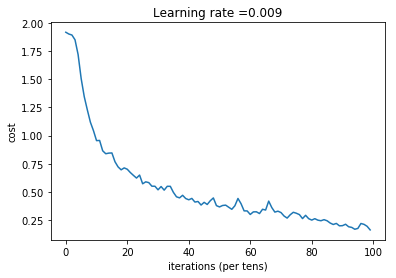
\includegraphics[width=0.6\textwidth]{course4/CONV_application}
\end{center}
\end{figure}

Congratulations! You have finised the assignment and built a model that recognizes SIGN language with almost 80\% accuracy on the test set. If you wish, feel free to play around with this dataset further. You can actually improve its accuracy by spending more time tuning the hyperparameters, or using regularization (as this model clearly has a high variance).

\clearpage